%% -*- coding: utf-8 -*-
\documentclass[12pt,a4paper]{scrartcl}
\usepackage[utf8]{inputenc}
\usepackage[english,russian]{babel}
\usepackage{indentfirst}
\usepackage{misccorr}
\usepackage{graphicx}
\usepackage{amsmath}
\usepackage[T1]{fontenc}
\usepackage{pbox}
\begin{document}
 \begin{center}
 {\hugeМетоды оптимизации\\
  Задание №1}
 \end{center}
 \begin{flushright}
{\large Сайков К.А\\ПМ-1801}
\end{flushright}
 \begin{flushleft}
  \LargeУсловие задания:
  \begin{center}
   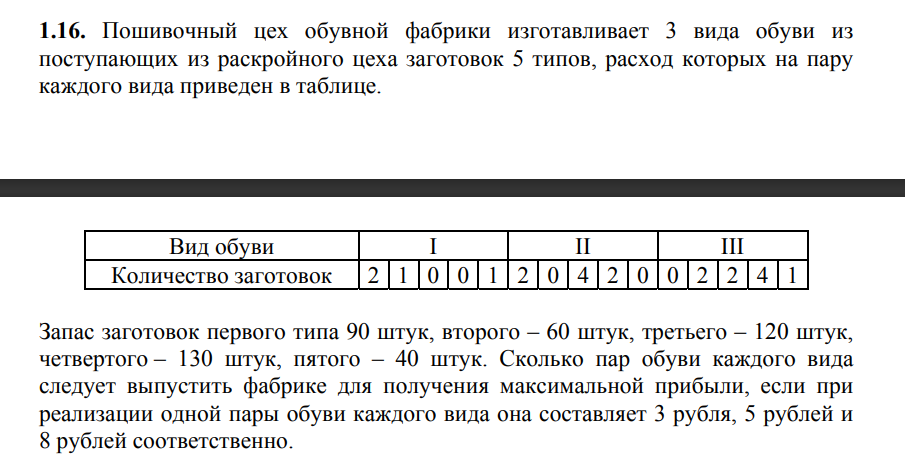
\includegraphics[scale=0.5]{conditions of the problem.png}
  \end{center}
 \end{flushleft}
 \begin{center}
  \begin{flushleft}
   \LargeРешение задания:\\
   \normalsizeЗапись в более удобном виде условий: \\ \\ \\
  \end{flushleft}
\begin{tabular}{ |c|c|c|c|c| }
 \hline
 \pbox
{50сm}{\centeringВид обуви\hline\centeringзаготовка}
 & I & II & III & Запасы заготовок\\
 \hline
  А & 2 & 2 & 0 & 90 \\
  \hline
  Б & 1 & 0 & 2 & 60 \\
  \hline
  В & 0 & 4 & 2 & 120 \\
  \hline
  Г & 0 & 2 & 4 & 130 \\
  \hline
  Д & 1 & 0 & 1 & 90 \\
  \hline
  Стоимость & 3 & 5 & 8 & - \\
 \hline
\end{tabular}
\end{center}
\begin{flushleft}
 Целевая функция\\
 f(x1,x2,x3) = 3*x1+5*x2+8*x3 \rightarrow min \\
 Ограничения составлены на основании таблицы выше\\
 \begin{tabular}
  x1+2*x3 <= 60 \\
  2*x1+2*x2 <= 90 \\
  4*x2+2*x3 <= 120 \\
  2*x2+4*x3 <= 130 \\
  x1+x2 <= 4 \\
  естественные ограничения \\
  x_{i}>=0\quad i = 1,2,3
 \end{tabular}
 \\Решение при помощи библиотеки cvxpy дало следующий результат:\\ x_{1} = 2\; x_{2} = 5.6\; f=-16.4
\end{flushleft}
\end{document}